% !TEX TS-program = XeLaTeX
% use the following command:
% all document files must be coded in UTF-8
\documentclass[portuguese]{textolivre}
% build HTML with: make4ht -e build.lua -c textolivre.cfg -x -u article "fn-in,svg,pic-align"

\journalname{Texto Livre}
\thevolume{16}
%\thenumber{1} % old template
\theyear{2023}
\receiveddate{\DTMdisplaydate{2022}{12}{12}{-1}} % YYYY MM DD
\accepteddate{\DTMdisplaydate{2023}{1}{9}{-1}}
\publisheddate{\DTMdisplaydate{2023}{1}{10}{-1}}
\corrauthor{Lauro Sérgio Machado Pereira}
\articledoi{10.1590/1983-3652.2023.42097}
%\articleid{36123} % if the article ID is not the last 5 numbers of its DOI, provide it using \articleid{} commmand
%\articleid{NNNN} % if the article ID is not the last 5 numbers of its DOI, provide it using \articleid{} commmand 
% list of available sesscions in the journal: articles, dossier, reports, essays, reviews, interviews, editorial
\articlesessionname{reviews}
\runningauthor{Pereira} 
%\editorname{Leonardo Araújo} % old template
\sectioneditorname{Daniervelin Pereira}
\layouteditorname{Daniervelin Pereira}

\title{Resenha: Formação docente em língua inglesa: diferentes perspectivas}
\othertitle{Review: Teacher education in English: different perspectives}
% if there is a third language title, add here:
%\othertitle{Artikelvorlage zur Einreichung beim Texto Livre Journal}

\author[1]{Lauro Sérgio Machado Pereira \orcid{0000-0002-7144-2733} \thanks{Email: \href{mailto:lauropereiraifnmg@gmail.com}{lauropereiraifnmg@gmail.com}}}

\affil[1]{Instituto Federal do Norte de Minas Gerais, Janaúba, MG, Brasil.}


\addbibresource{article.bib}
% use biber instead of bibtex
% $ biber article

% used to create dummy text for the template file
\definecolor{dark-gray}{gray}{0.35} % color used to display dummy texts
\usepackage{lipsum}
\SetLipsumParListSurrounders{\colorlet{oldcolor}{.}\color{dark-gray}}{\color{oldcolor}}

% used here only to provide the XeLaTeX and BibTeX logos
\usepackage{hologo}

% if you use multirows in a table, include the multirow package
\usepackage{multirow}

% provides sidewaysfigure environment
\usepackage{rotating}

% CUSTOM EPIGRAPH - BEGIN 
%%% https://tex.stackexchange.com/questions/193178/specific-epigraph-style
\usepackage{epigraph}
\renewcommand\textflush{flushright}
\makeatletter
\newlength\epitextskip
\pretocmd{\@epitext}{\em}{}{}
\apptocmd{\@epitext}{\em}{}{}
\patchcmd{\epigraph}{\@epitext{#1}\\}{\@epitext{#1}\\[\epitextskip]}{}{}
\makeatother
\setlength\epigraphrule{0pt}
\setlength\epitextskip{0.5ex}
\setlength\epigraphwidth{.7\textwidth}
% CUSTOM EPIGRAPH - END

% LANGUAGE - BEGIN
% ARABIC
% for languages that use special fonts, you must provide the typeface that will be used
% \setotherlanguage{arabic}
% \newfontfamily\arabicfont[Script=Arabic]{Amiri}
% \newfontfamily\arabicfontsf[Script=Arabic]{Amiri}
% \newfontfamily\arabicfonttt[Script=Arabic]{Amiri}
%
% in the article, to add arabic text use: \textlang{arabic}{ ... }
%
% RUSSIAN
% for russian text we also need to define fonts with support for Cyrillic script
% \usepackage{fontspec}
% \setotherlanguage{russian}
% \newfontfamily\cyrillicfont{Times New Roman}
% \newfontfamily\cyrillicfontsf{Times New Roman}[Script=Cyrillic]
% \newfontfamily\cyrillicfonttt{Times New Roman}[Script=Cyrillic]
%
% in the text use \begin{russian} ... \end{russian}
% LANGUAGE - END

% EMOJIS - BEGIN
% to use emoticons in your manuscript
% https://stackoverflow.com/questions/190145/how-to-insert-emoticons-in-latex/57076064
% using font Symbola, which has full support
% the font may be downloaded at:
% https://dn-works.com/ufas/
% add to preamble:
% \newfontfamily\Symbola{Symbola}
% in the text use:
% {\Symbola }
% EMOJIS - END

% LABEL REFERENCE TO DESCRIPTIVE LIST - BEGIN
% reference itens in a descriptive list using their labels instead of numbers
% insert the code below in the preambule:
%\makeatletter
%\let\orgdescriptionlabel\descriptionlabel
%\renewcommand*{\descriptionlabel}[1]{%
%  \let\orglabel\label
%  \let\label\@gobble
%  \phantomsection
%  \edef\@currentlabel{#1\unskip}%
%  \let\label\orglabel
%  \orgdescriptionlabel{#1}%
%}
%\makeatother
%
% in your document, use as illustraded here:
%\begin{description}
%  \item[first\label{itm1}] this is only an example;
%  % ...  add more items
%\end{description}
% LABEL REFERENCE TO DESCRIPTIVE LIST - END


% add line numbers for submission
%\usepackage{lineno}
%\linenumbers

\begin{document}
\maketitle

% \begin{quote}
%     \fullcite{nascimento_formacao_2019}
% \end{quote}

\begin{figure}[htbp]
 \centering
 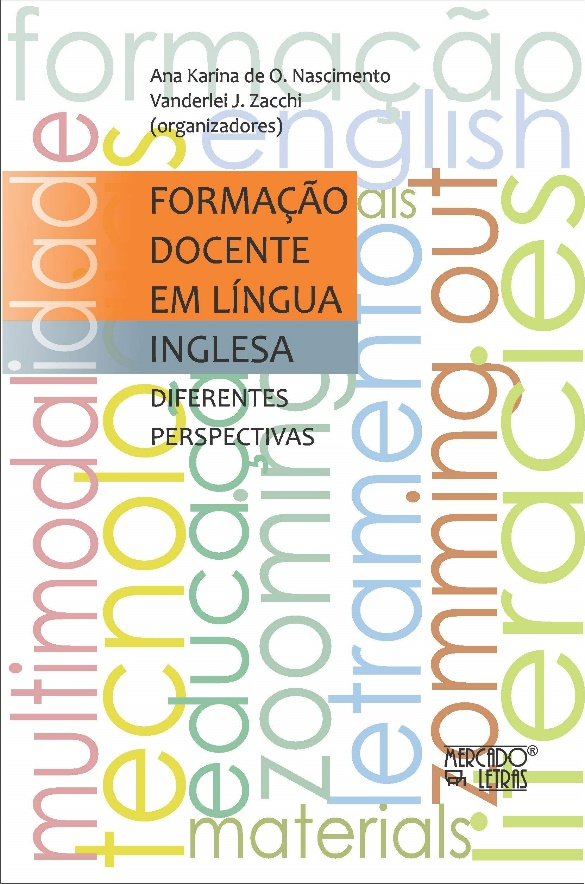
\includegraphics[width=0.5\textwidth]{Fig1.png}
 \caption*{\fullcite{nascimento_formacao_2019}.}
 %\caption{\fullcite{nascimento_formacao_2019}.}
 \label{fig01}
% \source{fonte.}
\end{figure}


A obra \textit{Formação docente em língua inglesa: diferentes perspectivas} reúne capítulos que versam sobre experiências de formação docente a partir de contextos diversos. Seus organizadores, Ana Karina de Oliveira Nascimento e Vanderlei José Zacchi, são doutores em Letras (Estudos Linguísticos e Literários em Inglês) pela Universidade de São Paulo (USP) e professores na Universidade Federal de Sergipe (UFS), onde atuam na graduação e na pós-graduação em Letras.

Os capítulos da coletânea são de autoria de professores participantes do projeto \textit{Formação Continuada de Professores de Inglês como Língua Adicional}. O projeto consistia em uma iniciativa de formação continuada de professores, que não se concretizou, do Ministério da Educação (MEC), com vistas a instrumentalizar criticamente professores de Língua Inglesa (LI) da educação básica para que formassem estudantes proficientes e atuantes no cenário da Copa do Mundo de Futebol (2014) e das Olimpíadas (2016) no Brasil. Assim sendo, ao se observar a impossibilidade de sua implementação, adaptou-se localmente a proposta em parceria com pesquisadores de universidades brasileiras. O projeto fez parte das atividades do Grupo de Pesquisa \textit{Letramentos em Inglês: língua, literatura e cultura} da UFS, que, por sua vez, agrega-se ao \textit{Projeto Nacional de Letramentos: Linguagem, Cultura, Educação e Tecnologia}, coordenado pelos professores Walkyria Monte Mór e Lynn Mario Trindade Menezes de Souza, ambos da USP. 

Conforme consta no prefácio da obra, escrito por Monte Mór e Menezes de Souza, devido aos baixos índices da educação brasileira e às deficiências nos programas de formação docente, é fundamental um projeto que possibilite as formações inicial e continuada caminharem juntas. Para tanto, é necessário conceber a profissionalização do docente de línguas sob uma ótica crítica. Ao tomarem a história das ideias pedagógicas no Brasil, os prefaciadores verificaram “a pertinência de haver uma política de ensino de línguas em escolas públicas, em consonância com um programa de formação docente, construindo reflexões e argumentos orientados pelas teorias de letramentos” (p. 10).

Segundo Monte Mór e Menezes de Souza, os membros do grupo procuraram “responder à indagação ‘Um Projeto de Educação Continuada deve continuar que educação’?” (p. 14), de modo que ao terem percebido a necessidade de ir além da formação tradicional já recebida, “estudaram sobre conceitos outros que se aproximam de questões educacionais da sociedade de hoje, desenharam práticas outras, buscaram um profissionalismo outro” (p. 14), considerando “o potencial da subjetividade de professores em formação inicial ou continuada” (p. 11). Na obra, “essas experiências e vivências são descritas, analisadas e compartilhadas com os leitores” (p. 14).

No primeiro capítulo, \textit{“English through new literacies”: analisando uma proposta de curso de formação (continuada) de professores de línguas}, Laudo Natel do Nascimento e Marlene de Almeida Augusto de Souza discutem “as práticas de aprendizagem e o desenvolvimento dos aspectos linguístico-discursivos da língua inglesa” (p. 24) a partir dos novos\footnote{O aspecto ‘novo’ implicou uma expansão da acepção convencional de letramento como habilidade de leitura e escrita, associada à ideia de alfabetização, no sentido de que passou “a considerar os aspectos socioideológicos inerentes às práticas de leitura” \cite[p. 21]{duboc_letramentos_2011}.} letramentos. Nesse sentido, refletem acerca da Língua Inglesa (LI) como prática social, associando aspectos linguísticos, educacionais e críticos conforme a proposta das Orientações Curriculares para o Ensino Médio (OCEM) \cite{brasil_orientacoes_2006}.

No segundo capítulo, \textit{Textos imagéticos em discussão: multimodalidade e letramento crítico em sala de aula de língua inglesa}, Gildete Cecília Neri Santos problematiza o trabalho com atividades de leitura mediante o uso de textos multimodais, os quais retiram o foco da escrita como único recurso de construção de sentidos, o que pode também ocorrer por meios visuais, sonoros e espaciais \cite{cope_multimodality_2003}. A autora compreende que “os textos se integram e produzem efeitos de sentido que vão além do que está escrito, ou seja, conseguem desenvolver seu letramento visual, a partir de um código semiótico” (p. 44).

No terceiro capítulo, \textit{Zooming in and out com professores de inglês}, Clarissa Menezes Jordão, Leina Jucá e Nara Takaki articulam três movimentos discursivos para se pensar a formação continuada (FC) de professores como um processo constante de negociação de sentidos, os quais estão condicionados a forças que estabilizam (centrípetas) e que deslocam (centrífugas) \cite{bakhtin_marxismo_1997}. As autoras problematizam a educação linguística em Língua Inglesa (LI) a partir da concepção de “língua como um organismo vivo” (p. 58) que torna possível a construção de sentidos na relação de aprendizagem do indivíduo com a realidade do mundo. Isso posto, consideram imprescindível tencionar a herança colonial moderna que posiciona a LI e suas culturas como superior a outras. 

No quarto capítulo, \textit{Da regra ao uso e do livro ao local: negociando práticas de linguagem na formação continuada}, Igor Gadioli e Flávio Soares Bezerra apresentam o trajeto de implementação de um curso de extensão \textit{on-line} voltado para práticas orais e escritas na educação linguística em LI. O curso abordou temas como o mito do falante nativo, a legitimidade local do uso da LI e de atividades de materiais didáticos, a importância de um currículo flexível, e o estilo dos diálogos nos livros didáticos de LI. Ao final da experiência de formação continuada, os autores consideram necessário balancear e negociar os objetivos do currículo idealizado pelos estudiosos da linguagem e as necessidades da realidade local.

No quinto capítulo, \textit{Professores-aprendizes e aprendizes-professores: materiais didáticos na formação continuada de professores de inglês}, Ana Karina de Oliveira Nascimento e Maria Amália Vargas problematizam “as possibilidades de uso de materiais didáticos de língua inglesa, com foco em livros do programa Nacional do Livro Didático (PNLD)” (p. 96). As pesquisadoras abordam o neoliberalismo no livro didático \cite{zacchi_neoliberalismo_2016} em diálogo com estudos referentes à multimodalidade \cite{cope_multimodality_2003}. Enfocam criticamente o tratamento dado pelos professores às imagens que constam no livro didático, uma vez que elas representam verdades que subjetivam os estudantes.

No sexto capítulo, \textit{“English language materials”: aproveitamento docente da formação continuada para o ensino de língua inglesa na rede pública de educação básica}, Thiago Domingos Freire discorre sobre as contribuições do curso de formação continuada em materiais de LI para suas práticas em sala de aula. Após problematizar a relação entre a escola e a comunidade externa acerca do uso de imagens, discutir o conceito ampliado de texto como construto ideológico e compartilhar uma experiência de aula com o livro didático, Freire destaca a contribuição dessa formação continuada para o desenvolvimento de uma postura e de uma atuação docentes mais críticas diante dos materiais aplicados à educação linguística.

No sétimo capítulo, \textit{Futuro e presente em formação: reflexões de graduandas em Letras sobre participação em um curso de formação continuada}, Clara Maria Correa Pereira Andrade, Nayara Stefanie Mandarino Silva e Raissa Amatori tecem considerações sobre sua participação no projeto \textit{Formação Continuada de Professores de Inglês como Língua Adicional}. As autoras relatam que, por meio da participação no curso, tiveram a oportunidade de entender melhor o papel problematizador do professor de línguas na educação linguística em contexto brasileiro, bem como ampliar os sentidos acerca da crítica na formação continuada de professores, pois é ela que possibilita o desenvolvimento de indivíduos autônomos e críticos.

No oitavo capítulo, \textit{Ensino-aprendizagem de inglês com tecnologias: o caso da formação continuada para professores de inglês em Sergipe}, Ana Flora Schlindwein, Denise Bértoli Braga e Paulo Boa Sorte apresentam objetivos, desenvolvimento e resultados do módulo sobre ensino-aprendizagem de inglês com tecnologias. Os autores refletem sobre as atividades desenvolvidas, de modo que suas considerações finais apontam para a necessidade de os gestores escolares se sensibilizarem para a elaboração de estratégias que possibilitem aos professores se engajar em atividades de formação continuada. Entre essas estratégias, tem-se desde a dispensa e a negociação de sábados letivos, até o incentivo financeiro pela participação.

No capítulo nove, \textit{Formação continuada de professores de LE (língua estrangeira) e um passeio pelo mundo das tecnologias: de onde partimos, para onde vamos?}, Mirela Magnani Pacheco primeiramente problematiza questões relativas à escola pública em conexão com as normativas da educação brasileira e com teorias sobre letramento digital, tecnologias e multimodalidade. Em seguida, trata da aplicação de tecnologias na aula de Língua estrangeira (LE), explicitando sugestões que englobam o uso de ferramentas mais tradicionais, como o quadro e as plataformas digitais, os jogos e os aplicativos em \textit{smartphones}. Reflete que é essencial investir na formação continuada de professores de LE para que esses profissionais criem possibilidades de uma educação linguística que usa criticamente as tecnologias digitais.

Por fim, no capítulo dez, \textit{Gamificação e ensino de língua inglesa}, Rogério Tenório de Azevedo narra o trabalho que realizou no curso de formação continuada de professores de LI, a fim de discutir conceitos teóricos de jogo, videogame, gamificação e novos letramentos, e indicar os benefícios dos jogos como prática social nas atividades didático-pedagógicas em LI na escola. Presenteia o leitor com três propostas de atividades práticas de gamificação, quais sejam: a transformação da escola em um jogo, a leitura de livros paradidáticos em LI e a aplicação das tecnologias ao ensino de LI. O autor argumenta a favor da necessidade de o professor de LI abordar a gamificação pelo viés crítico-reflexivo e associado às teorias dos novos letramentos, o que pode provocar mudanças de atitude nos estudantes.

Os capítulos da coletânea contribuem para a construção de um arcabouço teórico-prático que representa perspectivas inovadoras de formação continuada de professores de LI, uma vez que extrapolam a dimensão reflexiva e se atentam para as reais demandas das escolas públicas brasileiras. Dito de outra forma, é possível afirmar que a obra, em sua totalidade, constitui excelente exemplo de como, em tempos de profunda crise na política e na educação do país, se pode seguir “atuando nas brechas para contribuir com a formação continuada de professoras/es de inglês” \cite[p. 11]{pessoa_ousadia_2018}. 

Mediante discussão crítica acerca das teorias de letramentos, multiletramentos, novos letramentos, letramentos críticos, multimodalidade, tecnologia e gamificação, em diálogo com os documentos oficiais que regem a educação brasileira, os textos fornecem exemplos de estratégias e atividades que podem ser facilmente aplicadas pelos professores em seus contextos locais de trabalho.

A leitura da obra pode ser interessante para profissionais da educação em geral, mas principalmente para aqueles da área de Letras que pesquisam a formação continuada de professores de LI ou atuam como formadores de professores. Dado seu caráter de relato de experiências, o que contribui para o estabelecimento de uma conexão quase que afetiva com o leitor-professor, é altamente indicado que a obra possa ser lida e discutida em comunidades de prática com os pares. Em um cenário em que a formação continuada carece de investimentos, a obra resenhada apresenta um caminho possível a ser seguido por aqueles profissionais que acreditam e lutam por dias melhores para a educação linguística no Brasil.

\printbibliography\label{sec-bib}
% if the text is not in Portuguese, it might be necessary to use the code below instead to print the correct ABNT abbreviations [s.n.], [s.l.]
%\begin{portuguese}
%\printbibliography[title={Bibliography}]
%\end{portuguese}


\end{document}